\section{Illustration of Geometric Grouping}
\label{app:geometric-grouping}

\Cref{fig:geometric-grouping} illustrates \Cref{lem:kk-grouping}
with $k=2$ and $g=0.1$. The complete groups have total sizes
$2.85$, $2.10$, $2.00$, and $2.10$, respectively; each first reaches
the target $k$ at its last item. The remaining suffix $H$ has total
size $0.35<k$.

\begin{figure}[H]
    \centering
    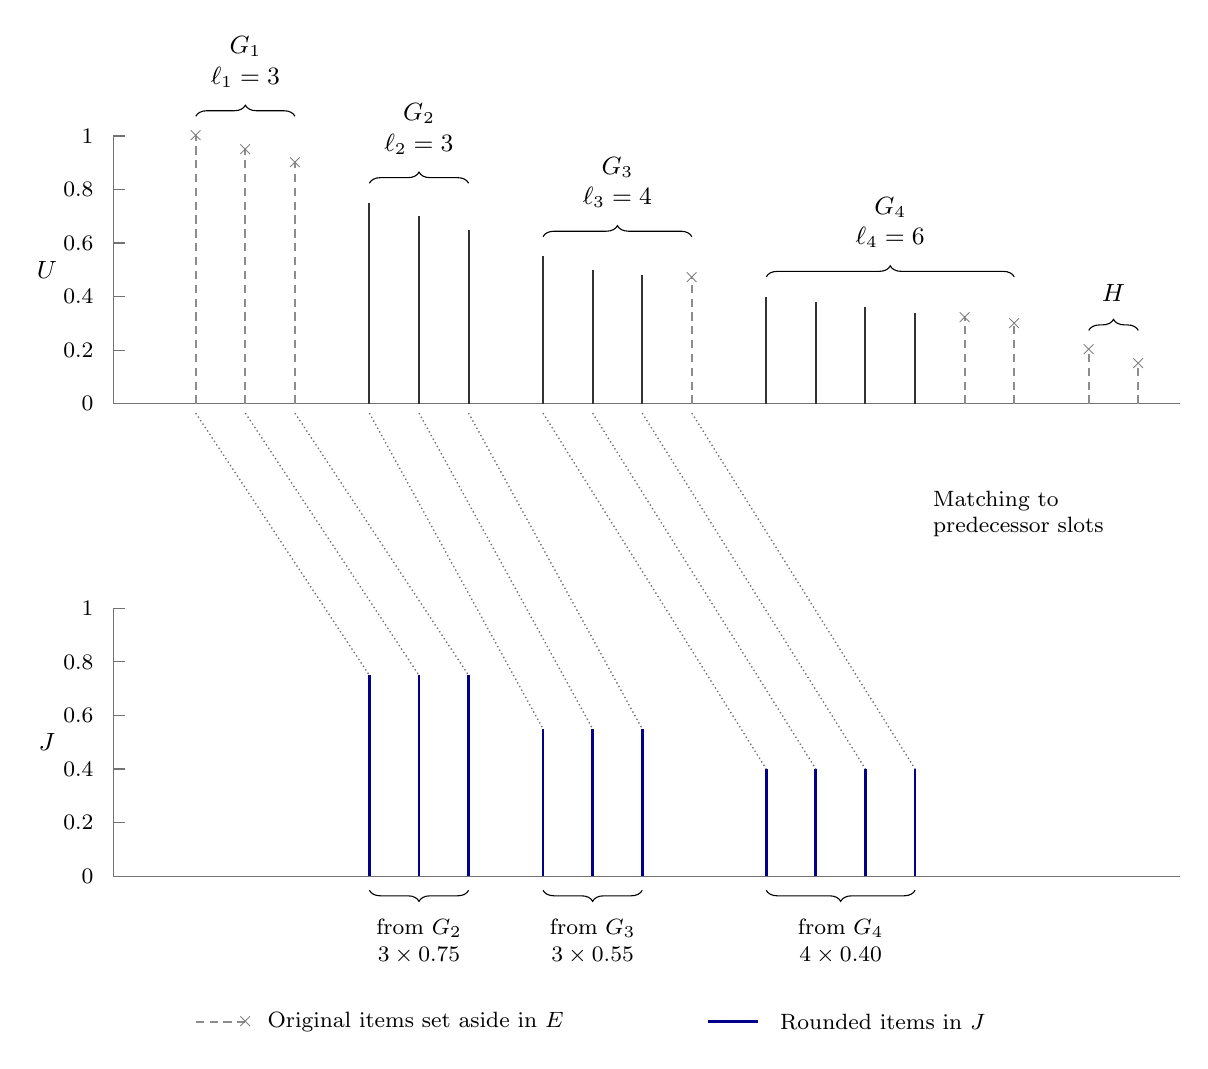
\begin{tikzpicture}[
        x=1.05cm, y=1cm,
        original/.style={black!80, line width=0.7pt},
        excluded/.style={black!45, densely dashed, line width=0.7pt},
        rounded/.style={blue!55!black, line width=1pt},
        matching/.style={black!55, densely dotted, line width=0.5pt},
        group brace/.style={decorate, decoration={brace, amplitude=4pt}},
        every node/.style={font=\small}
    ]
        % Item heights use the same scale in both panels.
        % Top baseline: 6 cm; one unit of item size: 3.4 cm.
        \foreach \base/\instance in {6/U,0/J} {
            \draw[black!55] (0,\base) -- (12.9,\base);
            \draw[black!55] (0,\base) -- (0,{\base+3.4});
            \foreach \tick in {0,0.2,0.4,0.6,0.8,1} {
                \draw[black!55] (0,{\base+3.4*\tick})
                    -- (0.15,{\base+3.4*\tick});
                \node[anchor=east, font=\footnotesize]
                    at (-0.12,{\base+3.4*\tick}) {$\tick$};
            }
            \node at (-0.8,{\base+1.7}) {$\instance$};
        }

        % Original items retained for rounding: G_2, G_3 minus its
        % smallest item, and G_4 minus its two smallest items.
        \foreach \x/\size in {
            3.1/0.75,3.7/0.70,4.3/0.65,
            5.2/0.55,5.8/0.50,6.4/0.48,
            7.9/0.40,8.5/0.38,9.1/0.36,9.7/0.34
        } {
            \draw[original] (\x,6) -- (\x,{6+3.4*\size});
        }

        % E consists of G_1, the trimmed items, and the suffix H.
        \foreach \x/\size in {
            1/1,1.6/0.95,2.2/0.90,
            7/0.47,10.3/0.32,10.9/0.30,11.8/0.20,12.4/0.15
        } {
            \draw[excluded] (\x,6) -- (\x,{6+3.4*\size});
            \node[font=\scriptsize, inner sep=0pt, text=black!55]
                at (\x,{6+3.4*\size}) {$\times$};
        }

        % Braces identify complete groups and their cardinalities.
        \foreach \left/\right/\height/\index/\count in {
            1/2.2/9.65/1/3,
            3.1/4.3/8.8/2/3,
            5.2/7/8.12/3/4,
            7.9/10.9/7.61/4/6
        } {
            \draw[group brace] (\left,\height) -- (\right,\height)
                node[midway, above=7pt, align=center]
                {$G_{\index}$\\$\ell_{\index}=\count$};
        }
        \draw[group brace] (11.8,6.93) -- (12.4,6.93)
            node[midway, above=7pt] {$H$};

        % Rounded items stay aligned with their retained originals.
        \foreach \x/\size in {
            3.1/0.75,3.7/0.75,4.3/0.75,
            5.2/0.55,5.8/0.55,6.4/0.55,
            7.9/0.40,8.5/0.40,9.1/0.40,9.7/0.40
        } {
            \draw[rounded] (\x,0) -- (\x,{3.4*\size});
        }

        % An injective matching from J to predecessor slots in U.
        % These connectors indicate domination, not item provenance.
        \foreach \slot/\item/\size in {
            1/3.1/0.75,1.6/3.7/0.75,2.2/4.3/0.75,
            3.1/5.2/0.55,3.7/5.8/0.55,4.3/6.4/0.55,
            5.2/7.9/0.40,5.8/8.5/0.40,6.4/9.1/0.40,7/9.7/0.40
        } {
            \draw[matching] (\slot,5.88) -- (\item,{3.4*\size});
        }
        \node[align=left, anchor=west, font=\footnotesize]
            at (9.8,4.6) {Matching to\\predecessor slots};

        \foreach \left/\right/\index/\copies/\size in {
            3.1/4.3/2/3/0.75,
            5.2/6.4/3/3/0.55,
            7.9/9.7/4/4/0.40
        } {
            \draw[group brace] (\right,-0.18) -- (\left,-0.18)
                node[midway, below=7pt, align=center, font=\footnotesize]
                {from $G_{\index}$\\$\copies\times\size$};
        }

        \draw[excluded] (1,-1.85) -- (1.6,-1.85);
        \node[font=\scriptsize, inner sep=0pt, text=black!55]
            at (1.6,-1.85) {$\times$};
        \node[anchor=west, font=\footnotesize] at (1.75,-1.85)
            {Original items set aside in $E$};
        \draw[rounded] (7.2,-1.85) -- (7.8,-1.85);
        \node[anchor=west, font=\footnotesize] at (7.95,-1.85)
            {Rounded items in $J$};
    \end{tikzpicture}
    \caption{Before and after geometric grouping. Each vertical line
    represents one item, with height equal to its size on the common
    scale. For $i\ge2$, retain $\ell_{i-1}$ items of $G_i$ and round
    them up to $\max G_i$, keeping them aligned beneath their originals.
    Dotted connections match these rounded
    items to distinct slots in $G_{i-1}$, illustrating $J\preceq U$.}
    \label{fig:geometric-grouping}
\end{figure}

Here $d_2=0$, $d_3=1$, and $d_4=2$. Thus
$D_3=\{0.47\}$ and $D_4=\{0.32,0.30\}$ are trimmed, giving
\[
    E=G_1\uplus D_3\uplus D_4\uplus H,
    \qquad
    J=\{0.75\times3,\;0.55\times3,\;0.40\times4\}.
\]
The first group supplies matching slots but contributes no rounded
items to $J$; its original items are packed separately in $E$.
